\vspace{-3mm}
\section{Senzorika}
\vspace{-3mm}
Mezi podstatné funkce trezoru patří jeho vnímání veličin jako čas, jeho náklon nebo okolní tlak.
Deska proto obsahuje tři nebo čtyři čipy (v~závislosti na dostupnosti součástek), které trezoru poskytují gyroskop, akcelerometr, 
magnetický kompas,
barometr, RTC a~také konektor pro připojení modulu GPS a~GPRS. Díky těmto funkcím může trezor poskytnout možnost ovládání 
pomocí různých gest. 
Trezor třeba může sloužit, s~využitím magnetického kompasu a~LED kruhu, jako kompas, nebo se dá využít akcelerometr, 
aby se dal trezor odemknout jen v~konkrétním náklonu. 

Všechny čipy zobrazené na obrázku \obr{fig:E4-sch_senzorika} komunikují s~ESP32 hlavně pomocí 
sběrnice I2C. Pro možnost zrychlení reakcí má však každý z~čipů také pin určený pro spuštění přerušení na procesoru, zapojení najdete na obrázku \obr{fig:E4-sch_senzorika}. 
To je užitečné, protože komunikaci na I2C řídí ESP32. Pokud se tedy ESP32 nerozhodne zeptat se jiného čipu 
na jím naměřená data, čip mu to po I2C nemá 
jak sdělit. Zároveň se však procesor nemůže bez ustání ptát na měření ostatních čipů, protože by pak nestíhal dělat nic jiného. Proto jsou čipy vybaveny 
pinem, který změní svou logickou hodnotu ve chvíli, kdy naměřené hodnoty splní nějaké podmínky. 
Například může být trezor naprogramován, aby se otevřel 
v~konkrétní čas. Tento čas se potom dá nastavit v~RTC jako hodnota, při jejímž dosažení RTC přepne pin přerušení. ESP32 pak jen přečte logickou hodnotu 
pinu a~vlastně ani nemusí komunikovat po I2C.

\paragraph{Akcelerometr, gyroskop a~magnetický kompas}
\addcontentsline{toc}{paragraph}{Akcelerometr gyroskom a~magnetický kompas}
Tyto funkce trezor má pro možnost sledování své pozice v~prostoru. 
Díky akcelerometru má trezor k~dispozici informaci o~směru a~velikosti svého zrychlení v~prostoru.
Gyroskop poskytuje informaci o~relativním natočení trezoru, což se může využít jako další podmínka pro otevření trezoru nebo pro různá ovládací gesta.
Magnetický kompas pak pochopitelně dodává informaci o~natočení vůči zemskému magnetickému poli.

Na prvním prototypu verze E4 poskytoval akcelerometr, gyroskop i~magnetický kompas čip \href{https://datasheet.lcsc.com/szlcsc/Bosch-Sensortec-BMX055_C94022.pdf}{BMX055} \parencite{bmx055},
protože však tento čip nebyl jednoduše dostupný, přidal jsem na další verzi i~čip \href{https://datasheet.lcsc.com/szlcsc/TDK-InvenSense-MPU-6050_C24112.pdf}{MPU6050} \parencite{mpu6050},
který obsahuje akcelerometr a~gyroskop a~čip \href{https://datasheet.lcsc.com/szlcsc/QST-QMC5883L-TR_C192585.pdf}{QMC5883} \parencite{qmc5883}, který dodává magnetický kompas.
Na desce je tak místo pro všechny tři čipy, a~pokud není k~dispozici BMX055, jednoduše se osadí MPU6050 a~QMC5883. 

\begin{figure}[h]
    \centering
    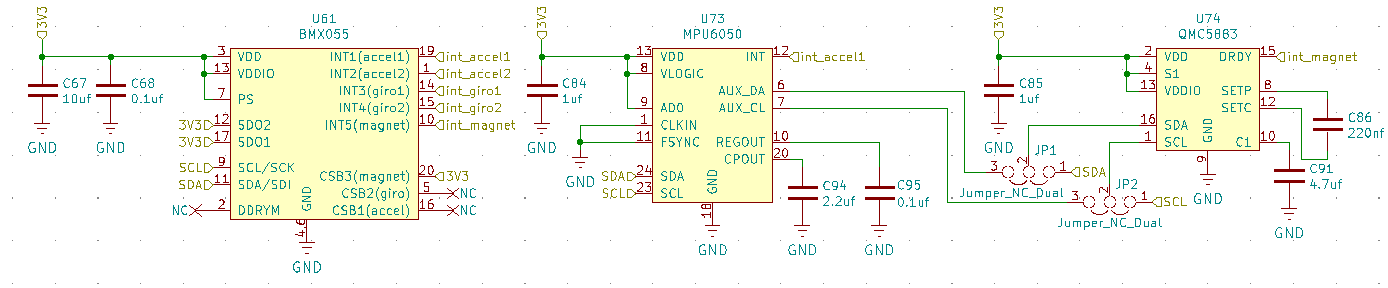
\includegraphics[width=\textwidth]{kapitoly/obrazky/E4/vnimani/BMX-MPU-QMC.png}
    \caption{Zapojení čipů BMX055, MPU6050 a~QMC5883}
    \label{fig:E4-9axis}
\end{figure}

\vspace{-5mm}

\subparagraph*{Akcelerometr}
\label{akcelerometr}
U~\ čipu \ BMX055 \ akcelerometr \ disponuje \ rozlišením \\ 1~mm$\cdot$s$^{-2}$ neboli 0,097m$g$ při rozsahu měření $\pm2g$. 
Jeho rozsah se ale dá nastavit, a~to na $\pm2g$, $\pm4g$, $\pm8g$, $\pm16g$, 
podle rozsahu se také mění přesnost měření. Přesnost je totiž omezena velikostí dvanáctibitového registru, do 
kterého se ukládají informace, a~při využívání většího 
rozsahu měření už tento registr není dostatečně velký, aby uchovával stejnou přesnost.

MPU6050 má vedle BMX u~akcelerometru stejné rozsahy měření, disponuje však šestnáctibitovými registry, a~tak je 
sto dosáhnout i~vetší přesnosti. Jeho maximální rozlišení je 
tak 60$\mu g$. Výměnou čipu BMX055 za čip MPU6050 jsem si tak polepšil i~po straně přesnosti, přesto, že tuto přesnost 
pravděpo\-dob\-ně nikdy BlackBox nevyužije. %todo jakože určitě ne ale přijde mi to divný zmiňovat i takhle mi to přijde jakési nekulantní ale možná je to zlozvyk z prezentace

\subparagraph*{Gyroskop}
\label{gyroskop}
U~čipu BMX055 je gyroskop sto poskytovat informaci o~úhlo\-vé rychlosti s~rozlišením na 0,004°\!/s,
 opět ale záleží na rozsahu měření kvůli stále stejné velikosti 
dvanáctibitového registru. 
Můžete si u~něj vybrat z~rozsahu $\pm125$°\!/s, $\pm250$°\!/s, $\pm500$°\!/s, $\pm1 000$°\!/s, $\pm2 000$°\!/s.

Po přechodu na čip MPU6050 jsem si opět po polepšil po straně přesnosti, i~u~gyroskopu totiž disponuje 
šestnáctibitovými registry a~rozsahy měření jsou opět stejné jako u~BMX055.

\subparagraph*{Magnetický kompas}
\label{magnetometr}
Čip BMX055 je sto měřit sílu magnetického pole s~přesností až na  0,3~$\mu$T 
v~rozsahu $\pm$1200~$\mu$T u~os $x$ a~$y$, u~osy $z$~pak v~rozsahu $\pm$2500~$\mu$T.

Magnetometr, který poskytuje čip QMC5883, pak měří v~rozsahu $\pm8$~Gs, což pro srovnání 
odpovídá $\pm$800~$\mu$T a~s~přesností až $2$~mGs opět pro srovnání to odpovídá $\pm$0,2~$\mu$T.
Na rozdíl od BMX055 se u~QMC5883 dá volit rozsah měření, a~tak si můžete vybrat z~$\pm2$~Gs 
a~nebo ze zmíněních $\pm8$~Gs.

%\newpage

\paragraph{Barometr, teploměr}
\addcontentsline{toc}{paragraph}{Barometr}
\label{barometr}
Barometr poskytuje informaci o~okolním atmosferickém tlaku. 
Tato informace může sloužit pro rozeznávání nadmořské výšky. 
BlackBox tak může sloužit i~jako jednoduchá meteorologická stanice, s~možností měření tlaku i~teploty (viz dále).

Od doby, kdy jsem z~nabídky JLCPCB vybíral čip 
\href{https://datasheet.lcsc.com/szlcsc/1907081118_Goertek-SPL06-007_C233787.pdf}{SPL06}, 
JLCPCB doplnilo do své nabídky několik dalších barometrů a~dneska bych tedy dost možná zvolil jiný. 
Každopádně tehdy jsem volil 
mezi dvěma čipy, které byly v~nabídce JLCPCB dostupné a~SPL06 měl vyšší rozlišení a~byl za téměř stejnou cenu.

SPL06 je sto měřit tlak v~rozsahu 950 až 1050~hPa s~přesností na 0,06~hPa 
a~je tak sto poznat změnu nadmořské výšky o~0,5~m.

SPL06 má také vedle barometru i~teploměr, který je sto měřit teplotu od -40°C do 85°C s~rozlišením na 0,01°C.

\begin{figure}[h]
    \centering
    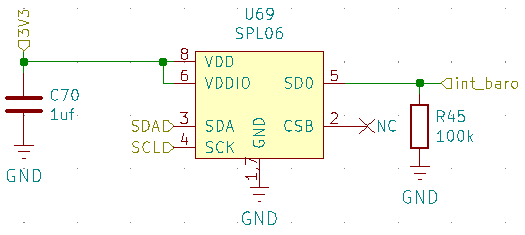
\includegraphics[width=\textwidth]{kapitoly/obrazky/E4/vnimani/SPL06.png}
    \caption{Zapojení čipu SPL06}
    \label{fig:E4-SPL06}
\end{figure}

\newpage

\paragraph{RTC}
\addcontentsline{toc}{paragraph}{RTC}
\label{RTC}
Aby si trezor mohl zachovávat povědomí o~aktuálním čase i~ve chvíli, kdy je vypnut, má k~dispozici čip 
\href{https://datasheet.lcsc.com/szlcsc/STMicroelectronics-M41T62Q6F_C113207.pdf}{M41T62} \parencite{m41t62}.

RTC je napájeno přímo z~baterie, hned za ochranou proti přepólování, aby bylo sto uchovávat čas i~ve vypnutém stavu.
Z~toho důvodu jistě potěší nízká spotřeba 350 nA ve chvíli, kdy jen uchovává čas a~35 µA ve chvíli, kdy je aktivní I2C.
Maximální odchylka od skutečného času může být 5~s~za měsíc provozu.

\begin{figure}[h]
    \centering
    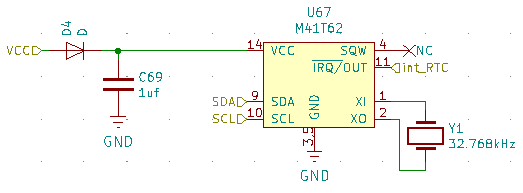
\includegraphics[width=\textwidth]{kapitoly/obrazky/E4/vnimani/RTC.png}
    \caption{Zapojení čipu M41T62}
    \label{fig:E4-M41T62}
\end{figure}

\newpage

\paragraph{Konektor pro GPS/GPRS modul}
\label{A9}
Ve chvíli, kdy jsem na trezor do\-pl\-ňo\-val čipy MPU6050 a~QMC5883, jsem zároveň doplnil i~tento konektor. 
Ve verzi, která je osazena MPU6050 a~QMC5883, a~nemá tedy osazen čip BMX055, 
je totiž více volných pinů. BMX055 totiž využívá pět pinů přerušení, zatím co MPU6050 a~QMC5883 mají každý po jednom. 
Proto při nevyužití BMX055 zbudou tři volné piny.
Protože čip A9G\footnote{Čip využívám jako GPS a~GPRS modul.} komunikuje po sběrnici UART, na rozdíl od ostatních čipu na desce. 
Pro UART však potřebuji
dva piny a~ty kolidují s~piny přerušení čipu BMX055. Proto se konektor dá použít, jen pokud není osazen BMX055.

\begin{figure}[h]
    \centering
    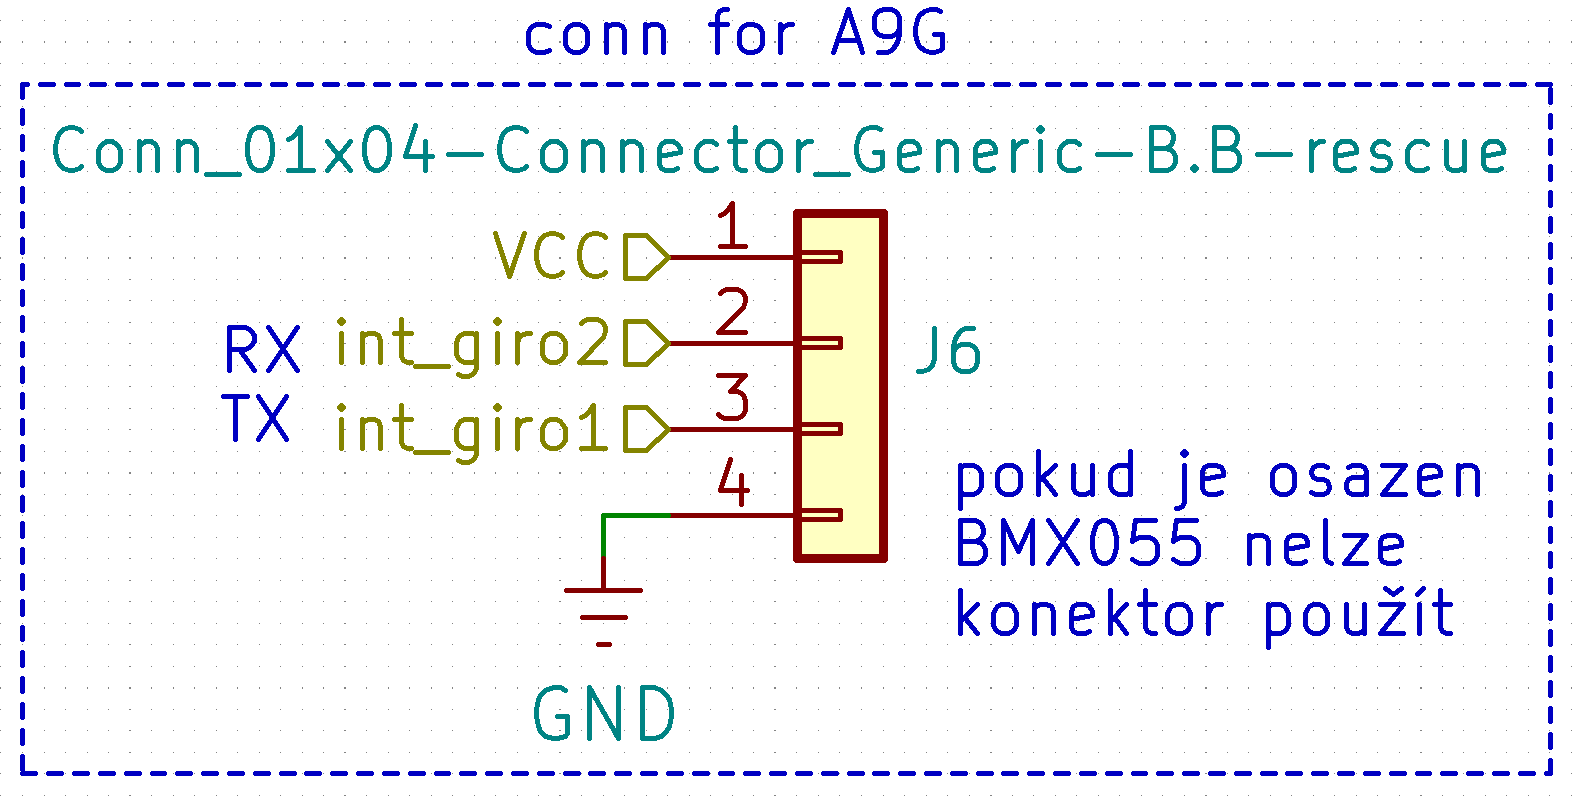
\includegraphics[width=\textwidth]{kapitoly/obrazky/E4/vnimani/conn-A9G.png}
    \caption{Zapojení konektoru pro A9G}
    \label{fig:E4-A9G}
\end{figure}

